\begin{abox}
	Quantum Mechanics
	\end{abox}
\begin{enumerate}
	\item A particle of energy $E$ scatters off a repulsive spherical potential
	$$
	V(r)=\left\{\begin{array}{ccc}
	V_{0} & \text { for } & r<a \\
	0 & \text { for } & r \leq a
	\end{array}\right.
	$$
	where $V_{0}$ and $a$ are positive constants. In the low energy limit, the total scattering crosssection is $\sigma=4 \pi a^{2}\left(\frac{1}{k a} \tanh k a-1\right)^{2}$, where $k^{2}=\frac{2 m}{h^{2}}\left(V_{0}-E\right)>0$. In the limit $V_{0} \rightarrow \infty$ the ratio of $\sigma$ to the classical scattering cross-section off a sphere of radius $a$ is
	{\exyear{NET/JRF(JUNE-2015)}}
\begin{tasks}(4)
\task[\textbf{A.}] 4
\task[\textbf{B.}] 3
\task[\textbf{C.}] 1
\task[\textbf{D.}] $\frac{1}{2}$
\end{tasks}
\begin{answer}
\begin{align*}
\sigma&=4 \pi a^{2}\left[\frac{1}{k a} \tanh k a-1\right]^{2}\\
k a \rightarrow \infty, \tanh k a \rightarrow 1 \Rightarrow \sigma&=4 \pi a^{2}\left(\frac{1}{k a}-1\right)^{2}\\
\text{	and }k a \rightarrow \infty, \lim _{k a \rightarrow \infty} \sigma_{H}&=4 \pi a^{2}\\
\text{classically }\sigma_{c}&=\pi a^{2}\\
\therefore \frac{\sigma_{H}}{\sigma_{c}}&=4
\end{align*}
So the correct answer is \textbf{Option (A)}
\end{answer}
\item A particle is scattered by a central potential $V(r)=V_{0} r e^{-\mu r}$, where $V_{0}$ and $\mu$ are positive constants. If the momentum transfer $\vec{q}$ is such that $q=|\vec{q}| \gg \mu$, the scattering crosssection in the Born approximation, as $q \rightarrow \infty$, depends on $q$ as
[You may use $\left.\int x^{n} e^{a x} d x=\frac{d^{n}}{d a^{n}} \int e^{a x} d x\right]$
{\exyear{NET/JRF(DEC-2016)}}
\begin{tasks}(4)
\task[\textbf{A.}] $q^{-8}$
\task[\textbf{B.}] $q^{-2}$
\task[\textbf{C.}] $q^{2}$
\task[\textbf{D.}] $q^{6}$
\end{tasks}
\begin{answer}
\begin{align*}
\intertext{The form factor is given for high energy as $q \rightarrow \infty$}
f(\theta, \phi)&=\frac{-2 m}{\hbar^{2} q} \int_{0}^{\infty} r V(r) \sin q r d r\\&=\frac{-2 m}{\hbar^{2} q} \int_{0}^{\infty} r^{2} V_{0} e^{-\mu v} \sin q r d r\\
&=\frac{-2 m}{\hbar^{2} q} V_{0} \int_{0}^{\infty} r^{2} e^{-\mu r} \frac{e^{i q r}-e^{-i q r}}{2 i} d r\\&=\frac{m V_{0}}{\hbar^{2} q} i\left[\int_{0}^{\infty} r^{2} e^{-r(\mu-i q)} d r-\int_{0}^{\infty} r^{2} e^{-r(\mu+i q)} d r\right]\\
&=\frac{m V_{0} i}{\hbar^{2} q}\left[\frac{\lfloor 2}{(\mu-i q)^{3}}-\frac{\lfloor 2}{(\mu+i q)^{3}}\right]\\&=\frac{2 m V_{0} i}{\hbar^{2} q}\left[\frac{\left((\mu+i q)^{3}-(\mu-i q)^{3}\right)}{(\mu+i q)^{3}(\mu-i q)^{3}}\right]\\
&=\frac{2 m V_{0}}{\hbar^{2} q} \frac{i\left[\left(\mu^{3}-i q^{3}+3 \mu^{2} i q-3 \mu q^{2}\right)-\left(\mu^{3}+i q^{3}-3 \mu^{2} i q-3 \mu q^{2}\right)\right]}{\left(\mu^{2}+q^{2}\right)^{3}}\\
&=\frac{2 m V_{0} i}{\hbar^{2} q}\left[\frac{6 \mu^{2} i q-2 i q^{3}}{\left(\mu^{2}+q^{2}\right)^{3}}\right]=\frac{2 m V_{0}}{\hbar^{2} q}\left[\frac{2 q^{3}-6 \mu^{2} q}{\left(\mu^{2}+q^{2}\right)^{3}}\right]\\
&\propto \frac{q^{3}}{q}\left(2-\frac{6 \mu^{2}}{q^{2}}\right) \times \frac{1}{q^{6}\left(\frac{\mu^{2}}{q^{2}}+1\right)^{3}} \propto q^{2} \times \frac{1}{q^{6}} \propto \frac{1}{q^{4}} \\&\left(\because \frac{\mu^{2}}{q^{2}}<<1\right)\\
&\sigma(\theta) \propto|f(\theta)|^{2} \propto\left(q^{-4}\right)^{2}=q^{-8}
\end{align*}
So the correct answer is \textbf{Option (A)}
\end{answer}	
\item A particle with incoming wave vector $\vec{k}$, after being scattered by the potential $V(r)=\frac{c}{r^{2}}$, goes out with wave vector $\vec{k}^{\prime}$. The differential scattering cross-section, calculated in the first Born approximation, depends on $q=\left|\vec{k}-\vec{k}^{\prime}\right|$, as
{\exyear{NET/JRF(JUNE-2020)}}
\begin{tasks}(2)
\task[\textbf{A.}] $1 / q^{2}$
\task[\textbf{B.}] $1 / q^{4}$
\task[\textbf{C.}]  $1 / q$
\task[\textbf{D.}] $1 / q^{3 / 2}$
\end{tasks}
\begin{answer}
\begin{align*}
\intertext{Using Born Approximation for high energy}
f(\theta)&=-\frac{2 m}{\hbar^{2} q} \int_{0}^{\infty} r V(r) \sin q r d r \quad\text{were} V(r)=\frac{c}{r^{2}}\\
f(\theta)&=-\frac{2 m c}{\hbar^{2} q} \int_{0}^{\infty} \frac{\sin q r}{r} d r\\&=-\frac{2 m c}{\hbar^{2} q} \frac{1}{2} \int_{-\infty}^{\infty} \frac{\sin q r}{r} d r\text{ solving from contour integration}\\
\int_{-\infty}^{\infty} \frac{\sin q r}{r} d r&=\frac{\pi}{2} \quad\text{ so }f(\theta) \propto \frac{1}{q} \Rightarrow D(\theta)\\&=|f(\theta)|^{2} \propto \frac{1}{q^{2}}
\end{align*}
So the correct answer is \textbf{Option (A)}
\end{answer}
\item The energy levels for a particle of mass $m$ in the potential $V(x)=\alpha|x|$, determined in the $W K B$ approximation
$$
\sqrt{2 m} \int_{a}^{b} \sqrt{E-V(x)} d x=\left(n+\frac{1}{2}\right) \hbar \pi
$$
(where $a, b$ are the turning points and $n=0,1,2 \ldots$ ), are
{\exyear{NET/JRF(JUNE-2016)}}
\begin{tasks}(2)
\task[\textbf{A.}] $E_{n}=\left[\frac{h \pi \alpha}{4 \sqrt{m}}\left(n+\frac{1}{2}\right)\right]^{\frac{2}{3}}$
\task[\textbf{B.}] $E_{n}=\left[\frac{3 h \pi \alpha}{4 \sqrt{2 m}}\left(n+\frac{1}{2}\right)\right]^{\frac{2}{3}}$
\task[\textbf{C.}] $E_{n}=\left[\frac{3 h \pi \alpha}{4 \sqrt{m}}\left(n+\frac{1}{2}\right)\right]^{\frac{2}{3}}$
\task[\textbf{D.}] $E_{n}=\left[\frac{h \pi \alpha}{4 \sqrt{2 m}}\left(n+\frac{1}{2}\right)\right]^{\frac{2}{3}}$
\end{tasks}
\begin{answer}$\left. \right. $
\begin{figure}[H]
	\centering
	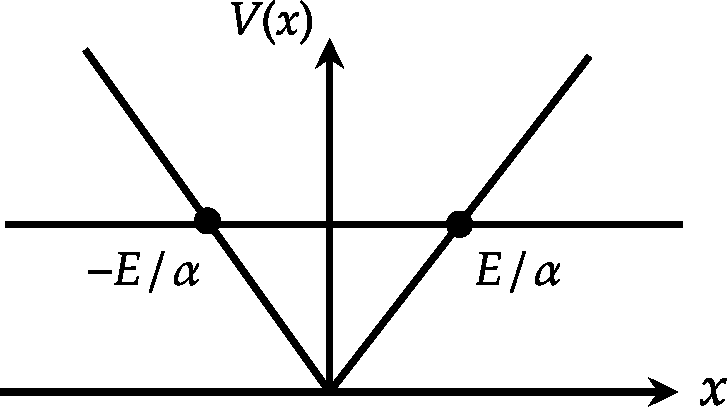
\includegraphics[height=3cm,width=5.5cm]{diagram-20210923(2)-crop}
\end{figure}
\begin{align*}
V(x)&=\alpha|x|\\
\Rightarrow V(x)&=\left\{\begin{array}{ll}-\alpha x, & x<0 \\ =\alpha x, & x>0\end{array}\right.\\
\sqrt{2 m} \int_{a}^{b} \sqrt{E-V(x)} d x&=\left(n+\frac{1}{2}\right) \pi \hbar\\
\text{From figure, }a&=\left(-\frac{E}{\alpha}\right), b=\left(\frac{E}{\alpha}\right) \Rightarrow \sqrt{2 m} \int_{-\frac{E}{\alpha}}^{\frac{E}{\alpha}} \sqrt{E-V(x)} d x\\&=\left(n+\frac{1}{2}\right) \pi \hbar\\
\text{From figure, }a&=\left(-\frac{E}{\alpha}\right), b=\left(\frac{E}{\alpha}\right) \Rightarrow \sqrt{2 m} \int_{-\frac{E}{\alpha}}^{\frac{E}{\alpha}} \sqrt{E-V(x)} d x\\&=\left(n+\frac{1}{2}\right) \pi \hbar\\
&\Rightarrow \sqrt{2 m} \int_{-\frac{E}{\alpha}}^{0} \sqrt{E+\alpha x} d x+\int_{0}^{\frac{E}{\alpha}} \sqrt{E-\alpha x} d x\\&=\left(n+\frac{1}{2}\right) \pi \hbar \Rightarrow 2 \sqrt{2 m} \int_{0}^{\frac{E}{\alpha}} \sqrt{E-\alpha x}(d x)=\left(n+\frac{1}{2}\right) \pi \hbar\\
\text{	put }E-\alpha x&=t\quad\quad
d x=-\frac{d t}{\alpha}\\
\text{	limit }&x \rightarrow 0 \Rightarrow t \rightarrow E, \quad \quad x \rightarrow \frac{E}{\alpha} \Rightarrow t \rightarrow 0\\
2 \sqrt{2 m} \int_{E}^{0} \sqrt{t}\left(\frac{-d t}{\alpha}\right)&=\left(n+\frac{1}{2}\right) \pi \hbar\\
2 \sqrt{2 m} \int_{E}^{0} \sqrt{t}\left(\frac{-d t}{\alpha}\right)&=\left(n+\frac{1}{2}\right) \pi \hbar\\
\Rightarrow-\frac{2 \sqrt{2 m}}{\alpha}\left[\frac{2}{3} t^{\frac{3}{2}}\right]_{E}^{0}&=\left(n+\frac{1}{2}\right) \pi \hbar \Rightarrow \frac{2 \sqrt{2 m}}{\alpha} \frac{2}{3} \cdot E^{\frac{3}{2}}\\&=\left(n+\frac{1}{2}\right) \pi h\\
\Rightarrow E^{\frac{3}{2}}&=\left(n+\frac{1}{2}\right) \frac{3 \pi \hbar \alpha}{4 \sqrt{2 m}} \Rightarrow E_{n}=\left[\frac{3 \hbar \pi \alpha}{4 \sqrt{2 m}}\left(n+\frac{1}{2}\right)\right]^{\frac{2}{3}}
\end{align*}
So the correct answer is \textbf{Option (B)}
\end{answer}	
\item The $n^{\text {th }}$ energy eigenvalues $E_{n}$ of a one-dimensional Hamiltonian $H=\frac{p^{2}}{2 m}+\lambda x^{4}$ (where $\lambda>0$ is a constant) in the WEB approximation, is proportional to
{\exyear{NET/JRF(JUNE-2018)}}
\begin{tasks}(2)
\task[\textbf{A.}] $\left(n+\frac{1}{2}\right)^{4 / 3} \lambda^{1 / 3}$
\task[\textbf{B.}] $\left(n+\frac{1}{2}\right)^{4 / 3} \lambda^{2 / 3}$
\task[\textbf{C.}] $\left(n+\frac{1}{2}\right)^{5 / 3} \lambda^{1 / 3}$
\task[\textbf{D.}] $\left(n+\frac{1}{2}\right)^{5 / 3} \lambda^{2 / 3}$
\end{tasks}
\begin{answer}
\begin{align*}
\intertext{From W.K.B approximation}\\
&4. \int_{0}^{x} P d x \propto\left(n+\frac{1}{2}\right) h\\
&4 \int_{0}^{\left(\frac{E}{\lambda}\right)^{1 / 4}} \sqrt{2 m\left(E-\lambda x^{4} d x\right)} \propto\left(n+\frac{1}{2}\right) h
\intertext{making the integration dimensional}
&4 \times(2 m E)^{1 / 2}\left(\frac{E}{\lambda}\right)^{1 / 4} \int_{0}^{1} \sqrt{1-t^{4}} d t \propto\left(n+\frac{1}{2}\right) \\&\Rightarrow E^{3 / 4} \propto\left(n+\frac{1}{2}\right) \lambda^{1 / 4} \Rightarrow E \propto\left(n+\frac{1}{2}\right)^{4 / 3} \lambda^{1 / 3}
\end{align*}
So the correct answer is \textbf{Option (A)}
\end{answer}	
\item The ground state energy of a particle of mass $m$ in the potential $V(x)=\frac{\hbar^{2} \beta}{6 m} x^{4}$ estimated using the normalized trial wavefunction $\psi(x)=\left(\frac{\alpha}{\pi}\right)^{\frac{1}{4}} e^{\frac{-\alpha x^{2}}{2}}$, is
$$
\text { [use } \left.\sqrt{\frac{\alpha}{\pi}} \int_{-\infty}^{\infty} d x x^{2} e^{-\alpha x^{2}}=\frac{1}{2 \alpha} \text { and } \sqrt{\frac{\alpha}{\pi}} \int_{-\infty}^{\infty} d x x^{4} e^{-\alpha x^{2}}=\frac{3}{4 \alpha^{2}}\right]
$$
{\exyear{NET/JRF(JUNE-2016)}}
\begin{tasks}(4)
\task[\textbf{A.}] $\frac{3}{2 m} \hbar^{2} \beta^{\frac{1}{3}}$
\task[\textbf{B.}] $\frac{8}{3 m} \hbar^{2} \beta^{\frac{1}{3}}$
\task[\textbf{C.}] $\frac{2}{3 m} \hbar^{2} \beta^{\frac{1}{3}}$
\task[\textbf{D.}] $\frac{3}{8 m} \hbar^{2} \beta^{\frac{1}{3}}$
\end{tasks}
\begin{answer}
\begin{align*}
\langle E\rangle&=\langle T\rangle+\langle V\rangle,\text{ for } \psi(x)=\left(\frac{\alpha}{\pi}\right)^{\frac{1}{4}} e^{-\frac{\alpha x^{2}}{2}},\langle T\rangle=\frac{\hbar^{2} \alpha}{4 m}\\
\langle V\rangle&=\left(\frac{\alpha}{\pi}\right)^{\frac{1}{2}} \int_{-\infty}^{\infty} \frac{\hbar^{2} \beta}{6 m} x^{4} e^{-\alpha x^{2}} d x=\left(\frac{\alpha}{\pi}\right)^{\frac{1}{2}} \frac{\hbar^{2} \beta}{6 m} \int_{-\infty}^{\infty} x^{4} e^{-\alpha x^{2}} d x\\&=\frac{\hbar^{2} \beta}{6 m} \cdot \frac{3}{4 \alpha^{2}}=\frac{\hbar^{2} \beta}{8 m \alpha^{2}}\\
\langle E\rangle&=\frac{\hbar^{2} \alpha}{4 m}+\frac{\hbar^{2} \beta}{8 m \alpha^{2}}\hspace{1.5cm}\text{(i)}\\
\frac{d E}{d \alpha}&=\frac{\hbar^{2}}{4 m}-\frac{2 \hbar^{2} \beta}{8 m \alpha^{3}}=0 \Rightarrow \frac{\hbar^{2}}{4 m}\left(1-\frac{\beta}{\alpha^{3}}\right)\\&=0 \Rightarrow \alpha=(\beta)^{\frac{1}{3}}
\intertext{Putting the value of $\alpha$ in equation (i),}
\langle E\rangle&=\frac{\hbar^{2}}{4 m}(\beta)^{\frac{1}{3}}+\frac{\hbar^{2} \beta}{8 m(\beta)^{\frac{2}{3}}}=\frac{\hbar^{2}}{4 m}\left[(\beta)^{\frac{1}{3}}+\frac{(\beta)^{\frac{1}{3}}}{2}\right]\\&=\frac{3}{8 m} \hbar^{2} \beta^{\frac{1}{3}}
\end{align*}
So the correct answer is \textbf{Option (D)}
\end{answer}	
\item Using the trial function
$$
\psi(x)=\left\{\begin{array}{cc}
A\left(a^{2}-x^{2}\right), & -a<x<a \\
0 & \text { otherwise }
\end{array}\right.
$$
the ground state energy of a one-dimensional harmonic oscillator is
{\exyear{NET/JRF(JUNE-2017)}}
\begin{tasks}(4)
\task[\textbf{A.}] $\hbar \omega$
\task[\textbf{B.}] $\sqrt{\frac{5}{14}} \hbar \omega$
\task[\textbf{C.}] $\frac{1}{2} \hbar \omega$
\task[\textbf{D.}] $\sqrt{\frac{5}{7}} \hbar \omega$
\end{tasks}
\begin{answer}
\begin{align*}
\psi(x)&=\left\{\begin{array}{ll}A\left(a^{2}-x^{2}\right), & -a<x<a \\ 0, & \text { otherwise }\end{array}\right.
\intertext{For normalization}
\int \psi^{*} \psi d x&=1\\
A^{2}&=\frac{15}{16 a^{5}} \Rightarrow A=\sqrt{\frac{15}{16 a^{5}}}\\
\langle T\rangle&=\frac{-\hbar^{2}}{2 m} \int_{-a}^{a} \psi^{*} \frac{\partial^{2}}{\partial x^{2}} \psi d x\\&=\frac{-\hbar^{2}}{2 m} \frac{15}{16 a^{5}} \cdot(-2)(2) \int_{0}^{a}\left(a^{2}-x^{2}\right) d x\\
\langle T\rangle&=\frac{5 \hbar^{2}}{4 m a^{2}}\\
\langle V\rangle&=\int_{-a}^{a} \psi^{*} V \psi d x,\text{ where }V(x)\\&=\frac{1}{2} m \omega^{2} x^{2}=\frac{1}{2} m \omega^{2} \frac{15}{16 a^{5}} 2 \int_{0}^{a} x^{2}\left(a^{2}-x^{2}\right)^{2} d x\\
\langle V\rangle&=\frac{m \omega^{2} a^{2}}{14}\\
E&=T+V=\frac{5 \hbar^{2}}{4 m a^{2}}+\frac{m \omega^{2} a^{2}}{14}\\
\frac{d E}{d a}&=0 \Rightarrow \frac{5 \times(-2) \hbar^{2}}{4 m a^{3}}+\frac{m \omega^{2} a}{7}=0 \Rightarrow a^{4}=\frac{35}{2}\left(\frac{\hbar^{2}}{m^{2} \omega^{2}}\right)\\
a^{2}&=\left(\frac{35}{2}\right)^{1 / 2}\left(\frac{\hbar}{m \omega}\right)\\
E&=\frac{5}{4} \times \frac{\hbar^{2}}{m} \cdot \frac{m \omega}{\hbar} \sqrt{\frac{2}{35}}+\frac{m \omega^{2}}{14} \sqrt{\frac{35}{2}} \frac{\hbar}{m \omega}\\
&=\frac{\hbar \omega}{2}\left(\frac{5}{2} \sqrt{\frac{2}{35}}+\frac{1}{7} \sqrt{\frac{35}{2}}\right)\\&=\frac{\hbar \omega}{2}\left(\sqrt{\frac{5}{14}}+\sqrt{\frac{5}{14}}\right)=\hbar \omega \sqrt{\frac{5}{14}}
\end{align*}
So the correct answer is \textbf{Option (B)}
\end{answer}	
\item The Coulomb potential $V(r)=-e^{2} / r$ of a hydrogen atom is perturbed by adding $H^{\prime}=b x^{2}$ (where $b$ is a constant) to the Hamiltonian. The first order correction to the ground state energy is\\
(The ground state wavefunction is $\left.\psi_{0}=\frac{1}{\sqrt{\pi a_{0}^{3}}} e^{-r / a_{0}}\right)$
{\exyear{NET/JRF(JUNE-2017)}}
\begin{tasks}(4)
\task[\textbf{A.}] $2 b a_{0}^{2}$
\task[\textbf{B.}] $b a_{0}^{2}$
\task[\textbf{C.}] $b a_{0}^{2} / 2$
\task[\textbf{D.}] $\sqrt{2} b a_{0}^{2}$
\end{tasks}
\begin{answer}
\begin{align*}
H^{\prime}&=b x^{2} \hspace{1.5cm}\text{ put }x=r \sin \theta \cos \phi\\
H^{\prime}&=b r^{2} \sin ^{2} \theta \cos ^{2} \phi\\
E_{1}^{1}&=\left\langle\psi_{1}\left|H^{\prime}\right| \psi_{1}\right\rangle,\left|\psi_{1}\right\rangle=\frac{1}{\sqrt{\pi a_{0}^{3}}} e^{-r / a_{0}}\\
&=\int \psi_{1}^{*} H^{\prime} \psi_{1} r^{2} \sin \theta d r d \theta d \phi\\
&=\frac{b}{\pi a_{0}^{3}} \int_{0}^{\infty} r^{2} e^{-\frac{2 r}{a_{0}}} r^{2} d r \int_{0}^{\pi} \sin ^{3} \theta d \theta \int_{0}^{2 \pi} \cos ^{2} \phi d \phi=b a_{0}^{2}
\end{align*}
So the correct answer is \textbf{Option (B)}
\end{answer}	
\item Consider a particle of mass $m$ in a potential $V(x)=\frac{1}{2} m \omega^{2} x^{2}+g \cos k x$. The change in the ground state energy, compared to the simple harmonic potential $\frac{1}{2} m \omega^{2} x^{2}$, to first order in $g$ is
{\exyear{NET/JRF(JUNE-2016)}}
\begin{tasks}(2)
\task[\textbf{A.}] $g \exp \left(-\frac{k^{2} \hbar}{2 m \omega}\right)$
\task[\textbf{B.}] $g \exp \left(\frac{k^{2} \hbar}{2 m \omega}\right)$
\task[\textbf{C.}] $g \exp \left(-\frac{2 k^{2} \hbar}{m \omega}\right)$
\task[\textbf{D.}] $g \exp \left(-\frac{k^{2} \hbar}{4 m \omega}\right)$
\end{tasks}
\begin{answer}
\begin{align*}
\intertext{Ground state wavefunction}
\psi_{0}(x)&=\left(\frac{m \omega}{\pi \hbar}\right)^{\frac{1}{4}} e^{-\frac{m \omega x^{2}}{2 \hbar}}\\
\text{The perturbation term is }H_{p}&=g \cos k x\\
\text{First order correction }E_{0}^{1}&=\int_{-\infty}^{\infty} \psi_{0}^{*}(x) H_{p} \psi_{0}(x) d x\\
&=\left(\frac{m \omega}{\pi \hbar}\right)^{\frac{1}{2}} g \int_{-\infty}^{\infty} e^{-\frac{m \omega x^{2}}{\hbar}}\left(\frac{e^{i k x}+e^{-i k x}}{2}\right) d x\\&=\frac{g}{2}\left(\frac{m \omega}{\pi \hbar}\right)^{\frac{1}{2}}\left[\int_{-\infty}^{\infty} e^{\frac{-m \omega x^{2}}{\hbar}} \cdot e^{i k x} d x+\int_{-\infty}^{\infty} e^{\frac{-m \omega x^{2}}{\hbar}} \cdot e^{-i k x} d x\right]\\
&=\frac{g}{2}\left(\frac{m \omega}{\pi \hbar}\right)^{\frac{1}{2}} \int_{-\infty}^{\infty} e^{-\frac{m \omega x^{2}}{\hbar}+i k x} d x+\frac{g}{2}\left(\frac{m \omega}{\pi \hbar}\right)^{\frac{1}{2}} \int_{-\infty}^{\infty} e^{\frac{-m \omega x^{2}}{\hbar}-i k x} d x
\intertext{From $1^{\text {st }}$ term, we have}
&=\frac{g}{2}\left(\frac{m \omega}{\pi \hbar}\right)^{\frac{1}{2}} \int_{-\infty}^{\infty} e^{-\frac{m \omega}{\hbar}\left[x^{2}+\frac{2 i k x \hbar}{2 m \omega}+\left(\frac{i k \hbar}{2 m \omega}\right)^{2}-\left(\frac{i k \hbar}{2 m \omega}\right)^{2}\right]} d x\\&=\frac{g}{2}\left(\frac{m \omega}{\pi \hbar}\right)^{\frac{1}{2}} \int_{-\infty}^{\infty} e^{-\frac{m \omega}{\hbar}\left(x+\frac{i k \hbar}{2 m \omega}\right)^{2}} e^{-\frac{k^{2} \hbar}{4 m \omega}} d x\\
&=\frac{g}{2} e^{-\frac{k^{2} \hbar}{4 m \omega}}\left(\frac{m \omega}{\pi \hbar}\right)^{\frac{1}{2}} \int_{-\infty}^{\infty} e^{\frac{m \omega}{\hbar}\left(x+\frac{i k \hbar}{2 m \omega}\right)^{2}} d x=e^{-\frac{k^{2} \hbar}{4 m \omega}}\\
\text{	Similarly, from term (ii), }&\frac{g}{2}\left(\frac{m \omega}{\pi \hbar}\right)^{\frac{1}{2}} \int_{-\infty}^{\infty} e^{\frac{m \omega x^{2}}{\hbar} i k x} d x\\
&=\frac{g}{2} e^{\frac{k^{2} h}{4 m \omega}}\left(\frac{m \omega}{\pi \hbar}\right)^{\frac{1}{2}} \int_{-\infty}^{\infty} e^{-\frac{m \omega}{\hbar}\left(x-\frac{i k \hbar}{2 m \omega}\right)^{2}} d x=e^{-\frac{k^{2} \hbar}{4 m \omega}}\\
\text{Hence, }E_{0}^{1}&=\frac{g}{2}\left[e^{-\frac{k^{2} \hbar}{4 m \omega}}+e^{\frac{k^{2} \hbar}{4 m \omega}}\right]=g e^{-\frac{k^{2} \hbar}{4 m \omega}}
\end{align*}
So the correct answer is \textbf{Option (D)}
\end{answer}	
\item The infinite square-well potential of a particle in a box of size a is modified as shown in the figure below (assume $\Delta<<a$ )\\
\begin{figure}[H]
	\centering
	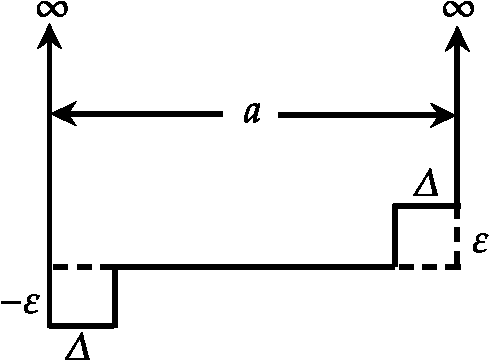
\includegraphics[height=3.5cm,width=5cm]{diagram-20211027(1)-crop}
\end{figure}
The energy of the ground state, compared to the ground state energy before the perturbation was added
{\exyear{NET/JRF(JUNE-2019)}}
\begin{tasks}(2)
\task[\textbf{A.}] Increases by a team of order $\varepsilon$
\task[\textbf{B.}] Decreases by a term of order $\varepsilon$
\task[\textbf{C.}] Increases by a term of order $\varepsilon^{2}$
\task[\textbf{D.}] Decreases by a term of order $\varepsilon^{2}$
\end{tasks}
\begin{answer}
\begin{align*}
\intertext{The perturbation is anti-symmetric about centre at box}
\mathrm{So} E_{1}^{1}&=0\\
E_{1}^{2}&=\sum_{m \neq 1} \frac{\left|\left\langle\varphi_{1}|w| \varphi_{m}\right\rangle\right|^{2}}{E_{1}^{0}-E_{m}^{0}}, E_{1}^{0}>E_{m}^{0}\text{ so } E_{1}^{2}<0
\end{align*}
So the correct answer is \textbf{Option (D)}
\end{answer}	
\item The normalized wavefunction of a particle in three dimensions is given by $\psi(r, \theta, \varphi)=\frac{1}{\sqrt{8 \pi a^{3}}} e^{-r / 2 a}$ where $a>0$ is a constant. The ratio of the most probable distance from the origin to the mean distance from the origin, is
[You may use $\left.\int_{0}^{\infty} d x x^{n} e^{-x}=n !\right]$
{\exyear{NET/JRF(DEC-2017)}}
\begin{tasks}(4)
\task[\textbf{A.}] $\frac{1}{3}$
\task[\textbf{B.}] $\frac{1}{2}$
\task[\textbf{C.}] $\frac{3}{2}$
\task[\textbf{D.}] $\frac{2}{3}$
\end{tasks}
\begin{answer}
\begin{align*}
\psi(r, \theta, \varphi)&=\frac{1}{\sqrt{8 \pi a^{3}}} e^{\frac{-r}{2 a}}\\
\langle r\rangle&=\iiint r \psi^{*} \psi r^{2} d r \sin \theta d \theta d \phi=\frac{3}{2}(2 a)=3 a
\intertext{one can compare the wave function at hydrogen atom with Bohr radius $a_{0}=2 a$ most probable distance,}
\frac{d}{d r} r^{2} e^{-r / a}&=0\\
r_{P}&=2 a\\
\frac{r_{p}}{\langle r\rangle}&=\frac{2 a}{3 a}=\frac{2}{3}
\end{align*}
So the correct answer is \textbf{Option (D)}
\end{answer}	
\item The state of an electron in a hydrogen atom is
$$
|\psi\rangle=\frac{1}{\sqrt{6}}|1,0,0\rangle+\frac{1}{\sqrt{3}}|2,1,0\rangle+\frac{1}{\sqrt{2}}|3,1,-1\rangle
$$
where $|n, l, m\rangle$ denotes common eigenstates of $\hat{H}, \hat{L}^{2}$ and $\hat{L}_{z}$ operators in the standard notation. In a measurement of $\hat{L}_{z}$ for the electron in this state, the result is recorded to be 0 . Subsequently a measurement of energy is performed. The probability that the result is $E_{2}$ (the energy of the $n=2$ state) is
{\exyear{NET/JRF(JUNE-2020)}}
\begin{tasks}(4)
\task[\textbf{A.}] 1
\task[\textbf{B.}] $1 / 2$
\task[\textbf{C.}] $2 / 3$
\task[\textbf{D.}]  $1 / 3$
\end{tasks}
\begin{answer}
\begin{align*}
\intertext{We will use postulates 4 first then use postulate 2 and 3.}
\intertext{If $L_{z}$ is measured and measurement is 0 then state is proportional to $\frac{1}{\sqrt{6}}|1,0,0\rangle+\frac{1}{\sqrt{3}}|2,1,0\rangle$}
P\left(E=E_{2}\right)&=\frac{\frac{1}{3}}{\frac{1}{6}+\frac{1}{3}}=\frac{\frac{1}{3}}{\frac{1+2}{6}}=\frac{\frac{1}{3}}{\frac{1}{2}}=\frac{2}{3}
\end{align*}
So the correct answer is \textbf{Option (C)}
\end{answer}	
\item An electron is in the ground state of a hydrogen atom. The probability that it is within the Bohr radius is approximately equal to
{\exyear{NET/JRF(JUNE-2014)}}
\begin{tasks}(4)
\task[\textbf{A.}] $0.60$
\task[\textbf{B.}] $0.90$
\task[\textbf{C.}]  $0.16$
\task[\textbf{D.}] $0.32$
\end{tasks}
\begin{answer}
\begin{align*}
\text{Probability: }\int_{0}^{a_{0}}\left|\frac{1}{\sqrt{\pi a_{0}^{3}}} e^{-r / a_{0}}\right|^{2} 4 \pi r^{2} d r&=\frac{4 \pi}{\pi a_{0}^{3}} \int_{0}^{a_{0}} r^{2} e^{-2 r / a_{0}} d r
\intertext{$=\frac{4}{a_{0}^{3}}\left\{\left[r^{2} e^{-2 r / a_{0}}\left(-\frac{a_{0}}{2}\right)\right]_{0}^{a_{0}}-\left[2 r\left(e^{-2 r / a_{0}}\right)\left(-\frac{a_{0}}{2}\right)\left(-\frac{a_{0}}{2}\right)\right]_{0}^{a_{0}}+\left[2 e^{-2 r / a_{0}}\left(-\frac{a_{0}}{2}\right)\left(-\frac{a_{0}}{2}\right)\left(-\frac{a_{0}}{2}\right)\right]_{0}^{\varphi_{0}}\right\}$}
\intertext{$=\frac{4}{a_{0}^{3}}\left[a_{0}^{2} e^{-\frac{2 a_{0}}{a_{0}}}\left(-\frac{a_{0}}{2}\right)-2 a_{0}\left(\frac{a_{0}^{2}}{4}\right) e^{-2 a_{0} / a_{0}}-\frac{a_{0}^{3}}{4} e^{-2 a_{0} / a_{0}}+2 e^{-0}\left(\frac{a_{0}^{3}}{8}\right)\right]$}\\
=\frac{4}{a_{0}^{3}}\left[-\frac{a_{0}^{3}}{2} \frac{1}{e^{2}}-\frac{a_{0}^{3}}{2} \frac{1}{e^{2}}-\frac{a_{0}^{3}}{4 e^{2}}+\frac{a_{0}^{3}}{4}\right]&=4\left[-\frac{5}{4 e^{2}}+\frac{1}{4}\right]=\left[-5 \times \frac{1}{e^{2}}+1\right]\\
&=[-5 \times 0.137+1]=[-0.685+1]=0.32
\end{align*}
So the correct answer is \textbf{Option (D)}
\end{answer}	
\item Let $\psi_{n l m}$ denote the eigenfunctions of a Hamiltonian for a spherically symmetric potential $V(r)$. The expectation value of $L_{2}$ in the state
$$
\psi=\frac{1}{6}\left[\psi_{200}+\sqrt{5} \psi_{210}+\sqrt{10} \psi_{21-1}+\sqrt{20} \psi_{211}\right] \text { is }
$$
{\exyear{NET/JRF(DEC-2013)}}
\begin{tasks}(4)
\task[\textbf{A.}] $-\frac{5}{18} \hbar$
\task[\textbf{B.}] $\frac{5}{6} \hbar$
\task[\textbf{C.}] $\hbar$
\task[\textbf{D.}] $\frac{5}{18} \hbar$
\end{tasks}
\begin{answer}
\begin{align*}
\left\langle L_{2}\right\rangle&=\left\langle\psi\left|L_{2}\right| \psi\right\rangle=\frac{1}{36} \times 0 \hbar+\frac{5}{36} \times 0 \hbar+\frac{10}{36} \times(-1 \hbar)+\frac{20}{36}(1 \hbar)\\&=\frac{10}{36} \hbar=\frac{5}{18} \hbar \quad \because\langle\psi \mid \psi\rangle=1
\end{align*}
So the correct answer is \textbf{Option (D)}
\end{answer}	
\item Spin $\frac{1}{2}$ fermions of mass $m$ and $4 m$ are in a harmonic potential $V(x)=\frac{1}{2} k x^{2}$. Which configuration of 4 such particles has the lowest value of the ground state energy?
{\exyear{NET/JRF(JUNE-2020)}}
\begin{tasks}(1)
\task[\textbf{A.}] 4 particles of mass $m$
\task[\textbf{B.}]  4 particles of mass $4 m$
\task[\textbf{C.}] 1 particle of mass $m$ and 3 particles of mass $4 m$
\task[\textbf{D.}] 2 particles of mass $m$ and 2 particles of mass $4 m$
\end{tasks}
\begin{answer}
\begin{align*}
V(x)&=\frac{1}{2} k x^{2}=\frac{1}{2} m \omega^{2} x^{2}\\
\text{For mass }m: V(x)&=\frac{1}{2} m \omega^{2} x^{2}\text{ and } E_{n}=\left(n+\frac{1}{2}\right) \hbar \omega\\
\text{For mass }4 m: V(x)&=\frac{1}{2}(4 m) \omega^{2} x^{2}=\frac{1}{2} m(2 \omega)^{2} x^{2}\\
\omega_{e f f}&=2 \omega \Rightarrow E_{n}=\left(n+\frac{1}{2}\right) \hbar(2 \omega)
\end{align*}
\begin{figure}[H]
	\centering
	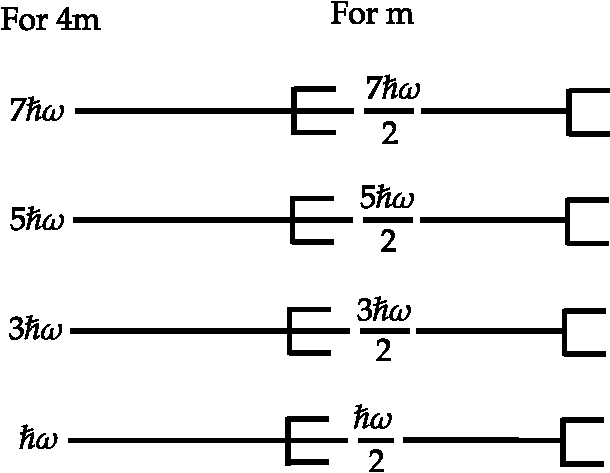
\includegraphics[height=6cm,width=8cm]{diagram-20211027(13)-crop}
\end{figure}
\begin{tasks}(2)
	\task[\textbf{A.}] $2\left(\frac{\hbar \omega}{2}\right)+2\left(\frac{3 \hbar \omega}{2}\right)=4 \hbar \omega$
	\task[\textbf{B.}]  $2(\hbar \omega)+2(3 \hbar \omega)=8 \hbar \omega$
	\task[\textbf{C.}] $\frac{\hbar \omega}{2}+2(\hbar \omega)+3 \hbar \omega=\frac{11}{2} \hbar \omega=5.5 \hbar \omega$
	\task[\textbf{D.}] $2\left(\frac{\hbar \omega}{2}\right)+2(\hbar \omega)=3 \hbar \omega$
\end{tasks}
$3 \hbar \omega$ is lowest among all 
So the correct answer is \textbf{Option (D)}
\end{answer}	
\item The Hamiltonian of a spin $\frac{1}{2}$ particle in a magnetic field $\vec{B}$ is given by $H=-\mu \cdot \vec{B} \cdot \vec{\sigma}$, where $\mu$ is a real constant and $\vec{\sigma}=\left(\sigma_{x}, \sigma_{y}, \sigma_{2}\right)$ are the Pauli spin matrices. If $\vec{B}=\left(B_{0}, B_{0}, 0\right)$ and the spin state at time $t=0$ is an eigenstate of $\sigma_{x}$, then of the expectation values $\left\langle\sigma_{x}\right\rangle,\left\langle\sigma_{y}\right\rangle$ and $\left\langle\sigma_{2}\right\rangle$
{\exyear{NET/JRF(JUNE-2018)}}
\begin{tasks}(2)
\task[\textbf{A.}] Only $\left\langle\sigma_{x}\right\rangle$ changes with time
\task[\textbf{B.}] Only $\left\langle\sigma_{y}\right\rangle$ changes with time
\task[\textbf{C.}] Only $\left\langle\sigma_{2}\right\rangle$ changes with time
\task[\textbf{D.}] All three change with time
\end{tasks}
\begin{answer}
\begin{align*}
\intertext{ $\left\langle\sigma_{x}\right\rangle,\left\langle\sigma_{y}\right\rangle$ and $\left\langle\sigma_{z}\right\rangle$ will changes with time because Eigen state of $\sigma_{x}$ ie $\frac{1}{\sqrt{2}}\left(\begin{array}{l}1 \\ 1\end{array}\right)$ and $\frac{1}{\sqrt{2}}\left(\begin{array}{c}1 \\ -1\end{array}\right)$ and can be written in basis of eigen state of $H=-\mu \cdot \vec{B} \cdot \vec{\sigma}=-B_{0}\left(\begin{array}{cc}0 & 1-i \\ 1+i & 0\end{array}\right)$}
\end{align*}
So the correct answer is \textbf{Option (D)}
\end{answer}	
\item A spin $-\frac{1}{2}$ particle is in the state $\chi=\frac{1}{\sqrt{11}}\left(\begin{array}{c}1+i \\ 3\end{array}\right)$ in the eigenbasis of $S^{2}$ and $S_{z} .$ If we measure $S_{z}$, the probabilities of getting $+\frac{h}{2}$ and $-\frac{h}{2}$, respectively are
{\exyear{NET/JRF(DEC-2013)}}
\begin{tasks}(4)
\task[\textbf{A.}] $\frac{1}{2}$ and $\frac{1}{2}$
\task[\textbf{B.}] $\frac{2}{11}$ and $\frac{9}{11}$
\task[\textbf{C.}] 0 and 1
\task[\textbf{D.}] $\frac{1}{11}$ and $\frac{3}{11}$
\end{tasks}
\begin{answer}
\begin{align*}
P\left(\frac{\hbar}{2}\right)&=\left|\frac{1}{\sqrt{11}}(10)\left(\begin{array}{c}1+i \\ 3\end{array}\right)\right|^{2}\\&=\frac{1}{11} \times 2=\frac{2}{11} \quad \because\langle\psi \mid \psi\rangle=1\\
P\left(-\frac{\hbar}{2}\right)&=\left|\frac{1}{\sqrt{11}}(01)\left(\begin{array}{c}1+i \\ 3\end{array}\right)\right|^{2}=\frac{9}{11}
\intertext{i.e. probability of $S_{2}$ getting $\left(\frac{\hbar}{2}\right)$ and $\left(-\frac{\hbar}{2}\right)$}
\end{align*}
So the correct answer is \textbf{Option (B)}
\end{answer}	
\item In a basis in which the $z$ - component $S_{z}$ of the spin is diagonal, an electron is in a spin state $\psi=\left(\begin{array}{c}(1+i) / \sqrt{6} \\ \sqrt{2 / 3}\end{array}\right) .$ The probabilities that a measurement of $S_{z}$ will yield the values $\hbar / 2$ and $-\hbar / 2$ are, respectively,
{\exyear{NET/JRF(JUNE-2013)}}
\begin{tasks}(4)
\task[\textbf{A.}] $1 / 2$ and $1 / 2$
\task[\textbf{B.}] $2 / 3$ and $1 / 3$
\task[\textbf{C.}] $1 / 4$ and $3 / 4$
\task[\textbf{D.}] $1 / 3$ and $2 / 3$
\end{tasks}
\begin{answer}
\begin{align*}
\intertext{Eigen state of $S_{z}$ is $\left|\phi_{1}\right\rangle=\left(\begin{array}{l}1 \\ 0\end{array}\right)$ and $\left|\phi_{2}\right\rangle=\left(\begin{array}{l}0 \\ 1\end{array}\right)$ corresponds to Eigen value $\frac{\hbar}{2}\text{}-\frac{\hbar}{2}$ respectively.}
P\left(\frac{\hbar}{2}\right)&=\frac{\left|\left\langle\phi_{1} \mid \psi\right\rangle\right|^{2}}{\langle\psi \mid \psi\rangle}=\left|\frac{1+i}{\sqrt{6}}\right|^{2}=\frac{2}{6}=\frac{1}{3}, \\ P\left(-\frac{\hbar}{2}\right)&=\frac{\left|\left\langle\phi_{2} \mid \psi\right\rangle\right|^{2}}{\langle\psi \mid \psi\rangle}=\frac{2}{3}
\end{align*}
So the correct answer is \textbf{Option (D)}
\end{answer}	
\item A particle moving in a central potential is described by a wavefunction $\psi(r)=z f(r)$ where $r=(x, y, z)$ is the position vector of the particle and $f(r)$ is a function of $r=|r|$
If $L$ is the total angular momentum of the particle, the value of $L^{2}$ must be
{\exyear{NET/JRF(JUNE-2019)}}
\begin{tasks}(4)
\task[\textbf{A.}] $2 \hbar^{2}$
\task[\textbf{B.}] $\hbar^{2}$
\task[\textbf{C.}] $4 \hbar^{2}$
\task[\textbf{D.}] $\frac{3}{4} \hbar^{2}$
\end{tasks}
\begin{answer}
\begin{align*}
\psi(r)&=z f(r)=r \cos \theta f(r)\\
\cos \theta&=P_{1}(\cos \theta) \Rightarrow l=1\\
\psi(r, \theta, \varphi)&=P_{1}(\cos \theta) r f(r)
\intertext{the measure at $L^{2}$ have eigen value}
l(l+1) \hbar^{2} \quad\text{ put }l&=1 \quad 1(l+1) \hbar^{2}=2 \hbar^{2}
\end{align*}
So the correct answer is \textbf{Option (A)}
\end{answer}	
\item Consider the normalized wavefunction
$$
\phi=a_{1} \psi_{11}+a_{2} \psi_{10}+a_{3} \psi_{1-1}
$$
where $\psi_{l m}$ is a simultaneous normalized eigenfunction of the angular momentum operators $L^{2}$ and $L_{z}$, with eigenvalues $l(l+1) \hbar^{2}$ and $m \hbar$ respectively. If $\phi$ is an eigenfunction of the operator $L_{x}$ with eigenvalue $\hbar$, then
{\exyear{NET/JRF(DEC-2014)}}
\begin{tasks}(2)
\task[\textbf{A.}] $a_{1}=-a_{3}=\frac{1}{2}, a_{2}=\frac{1}{\sqrt{2}}$
\task[\textbf{B.}] $a_{1}=a_{3}=\frac{1}{2}, \quad a_{2}=\frac{1}{\sqrt{2}}$
\task[\textbf{C.}] $a_{1}=a_{3}=\frac{1}{2}, \quad a_{2}=-\frac{1}{\sqrt{2}}$
\task[\textbf{D.}] $a_{1}=a_{2}=a_{3}=\frac{1}{\sqrt{3}}$
\end{tasks}
\begin{answer}
\begin{align*}
L_{x}|\phi\rangle&=\hbar|\phi\rangle \Rightarrow \frac{L_{+}+L_{-}}{2}|\psi\rangle=\lambda|\psi\rangle\\
\text{	For }L_{+}, \quad L_{+}\left[a_{1} \psi_{11}+a_{2} \psi_{10}+a_{3} \psi_{1-1}\right]&=a_{1} 0 \hbar \psi_{12}+a_{2} \sqrt{2} \hbar \psi_{11}+a_{3} \sqrt{2} \hbar \psi_{10}\\
&=a_{2} \sqrt{2} \hbar \psi_{11}+a_{3} \sqrt{2} \hbar \psi_{10}\\
\text{For }L_{-}, \quad L_{-}\left[a_{1} \psi_{11}+a_{2} \psi_{10}+a_{3} \psi_{1-1}\right]&=a_{1} \sqrt{2} \hbar \psi_{10}+a_{2} \sqrt{2} \hbar \psi_{1-1}\\
\text{Given }\frac{L_{+}+L_{-}}{2}|\phi\rangle&=\hbar|\phi\rangle\\
\Rightarrow \frac{L_{+}+L_{-}}{2}|\phi\rangle&=\frac{1}{2}\left[a_{2} \sqrt{2} \hbar \psi_{11}+\left(a_{1}+a_{3}\right) \sqrt{2} \hbar \psi_{10}+a_{2} \sqrt{2} \hbar \psi_{1-1}\right]\\
\because \frac{L_{+}+L_{-}}{2}|\phi\rangle&=\hbar\left[a_{1} \psi_{11}+a_{2} \psi_{10}+a_{3} \psi_{1-1}\right]\text{ (Given)}\\\text{Thus }\frac{a_{2}}{\sqrt{2}}=a_{1} \Rightarrow a_{2}&=\sqrt{2} a_{1}\\
\frac{a_{1}+a_{3}}{\sqrt{2}}&=a_{2} \Rightarrow \frac{a_{1}+a_{3}}{\sqrt{2}}=\sqrt{2} a_{1} \Rightarrow a_{1}=a_{3} \\& \because a_{1}^{2}+a_{2}^{2}+\frac{a_{2}^{2}}{2}=1\\
a_{1}&=a_{3}=\frac{1}{2}, a_{2}=\frac{1}{\sqrt{2}}
\end{align*}
So the correct answer is \textbf{Option (B)}
\end{answer}	
\item If $\hat{L}_{x}, \hat{L}_{y}, \hat{L}_{z}$ are the components of the angular momentum operator in three dimensions the commutator $\left[\hat{L}_{x}, \hat{L}_{x} \hat{L}_{y} \hat{L}_{z}\right]$ may be simplified to
{\exyear{NET/JRF(JUNE-2016)}}
\begin{tasks}(2)
\task[\textbf{A.}] $i \hbar L_{x}\left(\hat{L}_{z}^{2}-\hat{L}_{y}^{2}\right)$
\task[\textbf{B.}] $i \hbar \hat{L}_{z} \hat{L}_{y} \hat{L}_{x}$
\task[\textbf{C.}] $i \hbar L_{x}\left(2 \hat{L}_{z}^{2}-\hat{L}_{y}^{2}\right)$
\task[\textbf{D.}] 0
\end{tasks}
\begin{answer}
\begin{align*}
\left[L_{x}, L_{x} L_{y} L_{z}\right]&=L_{x}\left[L_{x}, L_{y} L_{z}\right]+\left[L_{x}, L_{x}\right] L_{y} L_{z}\\
&=L_{x}\left[L_{x}, L_{y}\right] L_{z}+L_{x} L_{y}\left[L_{x}, L_{z}\right]+0\\&=L_{x}\left[i \hbar L_{z}\right] L_{z}+L_{x} L_{y}\left(-i \hbar L_{y}\right)\\
&=i \hbar L_{x} L_{z}^{2}-i \hbar L_{x} L_{y}^{2}=i \hbar L_{x}\left(L_{z}^{2}-L_{y}^{2}\right)
\end{align*}
So the correct answer is \textbf{Option (A)}
\end{answer}	
\item The wavefunction of a particle of mass $m$, constrained to move on a circle of unit radius centered at the origin in the $x y$ - plane, is described by $\psi(\phi)=A \cos ^{2} \phi$, where $\phi$ is the azimuthal angle. All the possible outcomes of measurements of the $z$ - component of the angular momentum $L_{z}$ in this state, in units of $\hbar$ are
{\exyear{NET/JRF(DEC-2019)}}
\begin{tasks}(4)
\task[\textbf{A.}] $\pm 1$ and 0
\task[\textbf{B.}] $\pm 1$
\task[\textbf{C.}] $\pm 2$
\task[\textbf{D.}] $\pm 2$ and 0
\end{tasks}
\begin{answer}
\begin{align*}
\psi(\phi)&=A \cos ^{2} \phi=\frac{A}{2}(\cos 2 \phi+1)\\
&=\frac{A}{2}\left(\frac{e^{2 i \phi}+e^{-2 i \phi}}{2}+e^{0 i \phi}\right)\\
m&=2,-2,0
\end{align*}
So the correct answer is \textbf{Option (D)}
\end{answer}	
\item A particle of mass $m$ is in a cubic box of size $a$. The potential inside the box $(0 \leq x<a, 0 \leq y<a, 0 \leq z<a)$ is zero and infinite outside. If the particle is in an eigenstate of energy $E=\frac{14 \pi^{2} \hbar^{2}}{2 m a^{2}}$, its wavefunction is
{\exyear{NET/JRF(JUNE-2012)}}
\begin{tasks}(2)
\task[\textbf{A.}]  $\psi=\left(\frac{2}{a}\right)^{3 / 2} \sin \frac{3 \pi x}{a} \sin \frac{5 \pi y}{a} \sin \frac{6 \pi z}{a}$
\task[\textbf{B.}]  $\psi=\left(\frac{2}{a}\right)^{3 / 2} \sin \frac{7 \pi x}{a} \sin \frac{4 \pi y}{a} \sin \frac{3 \pi z}{a}$
\task[\textbf{C.}] $\psi=\left(\frac{2}{a}\right)^{3 / 2} \sin \frac{4 \pi x}{a} \sin \frac{8 \pi y}{a} \sin \frac{2 \pi z}{a}$
\task[\textbf{D.}] $\psi=\left(\frac{2}{a}\right)^{3 / 2} \sin \frac{\pi x}{a} \sin \frac{2 \pi y}{a} \sin \frac{3 \pi z}{a}$
\end{tasks}
\begin{answer}
\begin{align*}
E_{n_{x}, n_{y}, n_{2}}&=\left(n_{x}^{2}+n_{y}^{2}+n_{z}^{2}\right) \frac{\pi^{2} \hbar^{2}}{2 m a^{2}}\\&=\frac{14 \pi^{2} \hbar^{2}}{2 m a^{2}}\\
\Rightarrow n_{x}^{2}+n_{y}^{2}+n_{z}^{2}&=14 \Rightarrow n_{x}\\&=1, n_{y}=2, n_{z}=3
\end{align*}
So the correct answer is \textbf{Option (D)}
\end{answer}	
\item The energy of the first excited quantum state of a particle in the two-dimensional potential $V(x, y)=\frac{1}{2} m \omega^{2}\left(x^{2}+4 y^{2}\right)$ is
{\exyear{NET/JRF(DEC-2011)}}
\begin{tasks}(4)
\task[\textbf{A.}] $2 \hbar \omega$
\task[\textbf{B.}]  $3 \hbar \omega$
\task[\textbf{C.}] $\frac{3}{2} \hbar \omega$
\task[\textbf{D.}] $\frac{5}{2} \hbar \omega$
\end{tasks}
\begin{answer}
\begin{align*}
V(x, y)&=\frac{1}{2} m \omega^{2}\left(x^{2}+4 y^{2}\right)\\&=\frac{1}{2} m \omega^{2} x^{2}+\frac{1}{2} m 4 \omega^{2} y^{2}, E\\&=\left(n_{x}+\frac{1}{2}\right) \hbar \omega+\left(n_{y}+\frac{1}{2}\right) 2 \hbar \omega\\
\text{	For ground state energy }n_{x}&=0, n_{y}=0 \Rightarrow E\\&=\frac{\hbar \omega}{2}+\frac{1}{2} 2 \hbar \omega=\frac{3 \hbar \omega}{2}\\
\text{First exited state energy }n_{x}&=1, n_{y}=0 \Rightarrow \frac{3 \hbar \omega}{2}+\hbar \omega=\frac{5 \hbar \omega}{2}
\end{align*}
So the correct answer is \textbf{Option (D)}
\end{answer}	
\item A particle of mass $m$ moves in one dimension under the influence of the potential $V(x)=-\alpha \delta(x)$, where $\alpha$ is a positive constant. The uncertainty in the product $(\Delta x)(\Delta p)$ in its ground state is
{\exyear{NET/JRF(JUNE-2016)}}
\begin{tasks}(4)
\task[\textbf{A.}] $2 \hbar$
\task[\textbf{B.}] $\frac{\hbar}{2}$
\task[\textbf{C.}] $\frac{\hbar}{\sqrt{2}}$
\task[\textbf{D.}] $\sqrt{2} \hbar$
\end{tasks}
\begin{answer}
\begin{figure}[H]
	\centering
	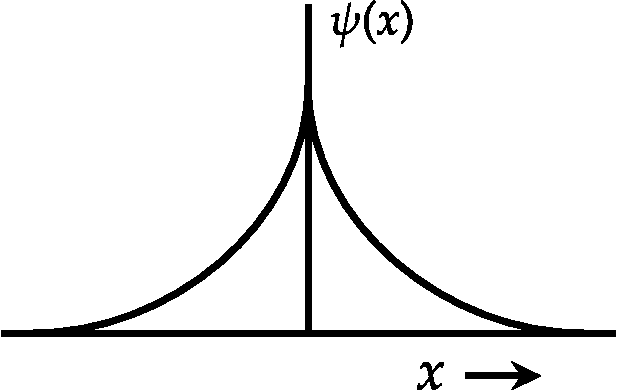
\includegraphics[height=3.5cm,width=5cm]{diagram-20210923(3)-crop}
\end{figure}
\begin{align*}
V(x)&=-\alpha \delta(x)
\intertext{For this potential wavefunction}
\psi(x)&=\left\{\begin{array}{ll}\sqrt{\alpha} e^{\alpha x}, & x<0 \\ \sqrt{\alpha} e^{-\alpha x}, & x>0\end{array}\right.
\intertext{which evenfunction about $x=0$}
\text{so }\langle x\rangle&=0,\langle p\rangle=0\\
\text{now }\left\langle x^{2}\right\rangle&=2 \alpha \int_{0}^{\infty} x^{2} e^{-2 \alpha x} d x=\frac{1}{2 \alpha^{2}} \Rightarrow \Delta x\\&=\sqrt{\left\langle x^{2}\right\rangle-\langle x\rangle^{2}}=\frac{1}{\sqrt{2} \alpha}\\
\left\langle p^{2}\right\rangle&=-\hbar^{2} \int_{-\infty}^{\infty} \psi^{*} \frac{d^{2}}{d x^{2}} \psi d x\\&=-\hbar^{2} \int_{-\infty}^{0} \sqrt{\alpha} e^{\alpha x} \frac{d^{2}}{d x^{2}} \sqrt{\alpha} e^{\alpha x} d x-\hbar^{2} \int_{0}^{\infty} \sqrt{\alpha} e^{-\alpha x} \frac{d^{2}}{d x^{2}} \sqrt{\alpha} e^{-\alpha x} d x\\
&=-\hbar^{2} \alpha^{3} \int_{-\infty}^{0} e^{2 \alpha x} d x-\hbar^{2} \alpha^{3} \int_{0}^{\infty} e^{-2 \alpha x} d x\\&=-\frac{\hbar^{2} \alpha^{3}}{2 \alpha}-\frac{\hbar^{2} \alpha^{3}}{2 \alpha}=-\hbar^{2} \alpha^{2}, \text{which is not possible}\\
\text{so, we will use the formula }\langle p\rangle^{2}&=\hbar^{2} \int_{-\infty}^{\infty}\left|\frac{d \psi}{d x}\right|^{2} d x=\hbar^{2} \alpha^{2}, \Delta p\\&=\sqrt{\left\langle p^{2}\right\rangle-\langle p\rangle^{2}}=\hbar \alpha\\
\text{now,}\Delta x \cdot \Delta p&=\frac{1}{\sqrt{2} \alpha} . \hbar \alpha=\frac{\hbar}{\sqrt{2}}
\end{align*}
So the correct answer is \textbf{Option (C)}
\end{answer}	
\item The motion of a particle of mass $m$ in one dimension is described by the Hamiltonian $H=\frac{p^{2}}{2 m}+\frac{1}{2} m \omega^{2} x^{2}+\lambda x .$ What is the difference between the (quantized) energies of the first two levels? (In the following, $\langle x\rangle$ is the expectation value of $x$ in the ground state)
{\exyear{NET/JRF(DEC-2013)}}
\begin{tasks}(4)
\task[\textbf{A.}] $\hbar \omega-\lambda\langle x\rangle$
\task[\textbf{B.}] $\hbar \omega+\lambda\langle x\rangle$
\task[\textbf{C.}] $\hbar \omega+\frac{\lambda^{2}}{2 m \omega^{2}}$
\task[\textbf{D.}] $\hbar \omega$
\end{tasks}
\begin{answer}
\begin{align*}
H&=\frac{p^{2}}{2 m}+\frac{1}{2} m \omega^{2} x^{2}+\lambda x \Rightarrow V(x)\\&=\frac{1}{2} m \omega^{2} x^{2}+\lambda x\\
V(x)&=\frac{1}{2} m \omega^{2}\left[x^{2}+\frac{2}{m \omega^{2}} \lambda x\right]\\&=\frac{1}{2} m \omega^{2}\left[x^{2}+2 \cdot x \cdot \frac{\lambda}{m \omega^{2}}+\frac{\lambda^{2}}{m^{2} \omega^{4}}-\frac{\lambda^{2}}{m^{2} \omega^{4}}\right]\\
V(x)&=\frac{1}{2} m \omega^{2}\left(x+\frac{\lambda}{m \omega^{2}}\right)^{2}-\frac{\lambda^{2}}{2 m \omega^{2}}\\
\therefore E_{n}&=\left(n+\frac{1}{2}\right) \hbar \omega-\frac{\lambda^{2}}{2 m \omega^{2}} \Rightarrow E_{1}-E_{0}\\&=\frac{3}{2} \hbar \omega-\frac{1}{2} \hbar \omega=\hbar \omega
\end{align*}
So the correct answer is \textbf{Option (D)}
\end{answer}	
\item The state vector of a one-dimensional simple harmonic oscillator of angular frequency $\omega$, at time $t=0$, is given by $|\psi(0)\rangle=\frac{1}{\sqrt{2}}[|0\rangle+|2\rangle]$, where $|0\rangle$ and $|2\rangle$ are the normalized ground state and the second excited state, respectively. The minimum time $t$ after which the state vector $|\psi(t)\rangle$ is orthogonal to $|\psi(0)\rangle$, is
{\exyear{NET/JRF(DEC-2017)}}
\begin{tasks}(4)
\task[\textbf{A.}] $\frac{\pi}{2 \omega}$ 
\task[\textbf{B.}] $\frac{2 \pi}{\omega}$
\task[\textbf{C.}] $\frac{\pi}{\omega}$
\task[\textbf{D.}] $\frac{4 \pi}{\omega}$
\end{tasks}
\begin{answer}
\begin{align*}
&\left\langle\psi(0)\left|=\frac{1}{\sqrt{2}}[|0\rangle+|2\rangle]\right.\right.\\
E_{2}&=\frac{5}{2} \hbar \omega \quad|\psi(t)\rangle=\frac{1}{\sqrt{2}}\left[|0\rangle e^{\frac{-\hbar \omega t}{2 \hbar}}+|2\rangle e^{\frac{-5 \hbar \omega t}{2} \hbar}\right]\\
E_{0}&=\frac{\hbar \omega}{2} \cdot\langle\psi(0) \psi \mid \psi(t)\rangle=0 \Rightarrow t=\frac{\hbar}{E_{2}-E_{0}} \cos ^{-1}(-1)\\
t&=\frac{\hbar}{\left(\frac{5 \hbar \omega}{2}-\frac{1}{2} \hbar \omega\right)} \cos ^{-1}(-1)=\frac{\hbar}{2 \hbar \omega / 2} \pi=\frac{\pi}{2 \omega}
\end{align*}
So the correct answer is \textbf{Option (A)}
\end{answer}	
\item Consider the normalized state $|\psi\rangle$ of a particle in a one-dimensional harmonic oscillator:
$$
|\psi\rangle=b_{1}|0\rangle+b_{2}|1\rangle
$$
where $|0\rangle$ and $|1\rangle$ denote the ground and first excited states respectively, and $b_{1}$ and $b_{2}$ are real constants. The expectation value of the displacement $x$ in the state $|\psi\rangle$ will be a minimum when
{\exyear{NET/JRF(JUNE-2013)}}
\begin{tasks}(4)
\task[\textbf{A.}] $b_{2}=0, b_{1}=1$
\task[\textbf{B.}] $b_{2}=\frac{1}{\sqrt{2}} b_{1}$
\task[\textbf{C.}] $b_{2}=\frac{1}{2} b_{1}$
\task[\textbf{D.}] $b_{2}=b_{1}$
\end{tasks}
\begin{answer}
\begin{align*}
\langle x\rangle&=b_{1}^{2}\langle 0|x| 0\rangle+b_{2}^{2}\langle 1|x| 1\rangle+2 b_{1} b_{2}\langle 0|x| 1\rangle\\
\text{	Since }\langle 0|x| 0\rangle&=0\text{ and }\langle 1|x| 1\rangle\\&=0 \Rightarrow\langle x\rangle=2 b_{1} b_{2}\langle 0|x| 1\rangle\\
\intertext{Min of $\langle x\rangle$ means $\min 2 b_{1} b_{2}$. We know that $b_{1}^{2}+b_{2}^{2}=1$}
\langle x \rangle_{min}&=\left[ \left( b_1+b_2\right)^2 -\left( b_1^2+b_2^2\right) \right] \bra{0}x\ket{1}\\&=\left[ \left( b_1+b_2\right)^2-1 \right] \bra{0}x\ket{1}\Rightarrow\left[1-\left( b_1-b_2\right)^2  \right] \bra{0}x
\ket{1}
\intertext{will be minimum and minimum value of $\left[1-\left(b_{1}-b_{2}\right)^{2}\right]$, there must be maximum of $\left(b_{1}-b_{2}\right)^{2}$, so $\Rightarrow b_{1}=b_{2}$}
\end{align*}
So the correct answer is \textbf{Option (D)}
\end{answer}
\item Let $|n\rangle$ denote the energy eigenstates of a particle in a one-dimensional simple harmonic potential $V(x)=\frac{1}{2} m \omega^{2} x^{2}$. If the particle is initially prepared in the state $|\psi(t=0)\rangle=\sqrt{\frac{1}{2}}(|0\rangle+|1\rangle)$, the minimum time after which the oscillator will be found in the same state is
{\exyear{NET/JRF(JUNE-2020)}}
\begin{tasks}(4)
\task[\textbf{A.}] $3 \pi /(2 \omega)$
\task[\textbf{B.}] $\pi / \omega$
\task[\textbf{C.}] $\pi /(2 \omega)$
\task[\textbf{D.}] $2 \pi / \omega$
\end{tasks}
\begin{answer}
\begin{align*}
|\psi(t=0)\rangle&=\sqrt{\frac{1}{2}}(|0\rangle+|1\rangle), \\|\psi(t=t)\rangle&=\sqrt{\frac{1}{2}}\left(|0\rangle e^{-\frac{i \omega t}{2}}+|1\rangle e^{-\frac{i 3 \omega x}{2}}\right)\\
|\langle\psi(t) \mid \psi(0)\rangle|^{2}&=1 \Rightarrow\left|\frac{1}{2}\left(\exp -\frac{i \omega t}{2}+\exp -\frac{3 i \omega t}{2}\right)\right|^{2}=1\\
|1+\exp (-i \omega t)|^{2}&=4 \Rightarrow t=\frac{2 \pi}{\omega}
\end{align*}
So the correct answer is \textbf{Option (D)}
\end{answer}	
\item A particle in the infinite square well potential
$$
V(x)=\left\{\begin{array}{lll}
0 & , & 0<x<a \\
\infty & , & \text { otherwise }
\end{array}\right.
$$
is prepared in a state with the wavefunction
$$
\psi(x)=\left\{\begin{array}{ll}
A \sin ^{3}\left(\frac{\pi x}{a}\right), & 0<x<a \\
0 & \text { otherwise }
\end{array}\right.
$$
The expectation value of the energy of the particle is
{\exyear{NET/JRF(JUNE-2014)}}
\begin{tasks}(4)
\task[\textbf{A.}] $\frac{5 \hbar^{2} \pi^{2}}{2 m a^{2}}$
\task[\textbf{B.}]  $\frac{9 \hbar^{2} \pi^{2}}{2 m a^{2}}$
\task[\textbf{C.}] $\frac{9 \hbar^{2} \pi^{2}}{10 m a^{2}}$
\task[\textbf{D.}] $\frac{\hbar^{2} \pi^{2}}{2 m a^{2}}$
\end{tasks}
\begin{answer}
\begin{align*}
\intertext{	$V(x)=\left\{\begin{array}{ll}0, & 0<x<a \\ \infty, & \text { otherwise }\end{array} \quad \psi(x)=\left\{\begin{array}{ll}A \sin ^{3}\left(\frac{\pi x}{a}\right), & 0<x<a \\ 0 & , \text { otherwise }\end{array}\right\}\right.$}
\psi(x)&=A \sin ^{3}\left(\frac{\pi x}{a}\right)=A \frac{3}{4} \sin \frac{\pi x}{a}-A \frac{1}{4} \sin \frac{3 \pi x}{a} \\&\left(\because \sin 3 A=3 \sin A-4 \sin ^{3} A\right)\\
&=\frac{A}{4}\left[\sqrt{\frac{a}{2}} \sqrt{\frac{2}{a}} \times 3 \sin \frac{\pi x}{a}-\sqrt{\frac{a}{2}} \sqrt{\frac{2}{a}} \sin \frac{3 \pi x}{a}\right] \Rightarrow \psi(x)\\&=\frac{A}{4}\left[3 \sqrt{\frac{a}{2}} \phi_{1}(x)-\sqrt{\frac{a}{2}} \phi_{3}(x)\right]\\
\langle\psi \mid \psi\rangle&=1 \Rightarrow 9 \frac{a}{32} A^{2}+\frac{a}{32} A^{2}=1 \Rightarrow \frac{10 a}{32} A^{2}\\&=1 \Rightarrow A=\sqrt{\frac{32}{10 a}}\\
\psi(x)&=\frac{1}{4}\left(3 . \sqrt{\frac{a}{2}} \sqrt{\frac{32}{10 a}} \phi_{1}(x)-\sqrt{\frac{a}{2}} \sqrt{\frac{32}{10 a}} \phi_{3}(x)\right)\\&=\frac{3}{\sqrt{10}} \phi_{1}(x)-\frac{1}{\sqrt{10}} \phi_{3}(x)\\
\text{Now, }\quad E_{1}&=\frac{\pi^{2} \hbar^{2}}{2 m a^{2}}, \quad E_{3}=\frac{9 \pi^{2} \hbar^{2}}{2 m a^{2}} \Rightarrow\langle E\rangle=a_{n} P\left(a_{n}\right)\\
\text{	Probability }P\left(E_{1}\right)&=\frac{\left|\left\langle\varphi_{1} \mid \psi\right\rangle\right|^{2}}{\langle\psi \mid \psi\rangle}=\frac{9}{10}, P\left(E_{3}\right)=\frac{\left|\left\langle\phi_{2} \mid \psi\right\rangle\right|^{2}}{\langle\psi \mid \psi\rangle}=\frac{1}{10}\\
\langle E\rangle&=\frac{9}{10} \times \frac{\pi^{2} \hbar^{2}}{2 m a^{2}}+\frac{1}{10} \times \frac{9 \pi^{2} \hbar^{2}}{2 m a^{2}} \Rightarrow\langle E\rangle=\frac{9 \pi^{2} \hbar^{2}}{10 m a^{2}}
\end{align*}
So the correct answer is \textbf{Option (C)}
\end{answer}	
\end{enumerate}